\chapter{研究背景}\label{chap:background}

本章では、本研究の背景について述べる。

\section{計算資源としての人}\label{ux8a08ux7b97ux8cc7ux6e90ux3068ux3057ux3066ux306eux4eba}

コンピュータのみでは解決が困難な問題を、人間を計算資源として利用することによって解決する考え方は
ヒューマンコンピュテーション\cite{humancomputation}と呼ばれる。
コンピュータは優れた処理能力を有するが、パターン認識能力など人間のほうが得意な処理分野は多く存在する。
これらの分野において人間とコンピュータがお互いの得意な領域において力を発揮することによって、
今までは実現が困難であったような処理でも実現することが可能となった。

ヒューマンコンピュテーションの例として挙げられるシステムとして、reCAPTCHA\cite{recaptcha}が存在する。
reCAPTCHAは、人間かコンピュータを識別するためのテストとして活用されているCAPTCHA\cite{captcha}を応用し、
識別を行いながらコンピュータでは識別できなかった文字の認識を人間に実行させるシステムだ。
reCAPTCHAによって、人は自分が人間であることを証明しながら、紙の本のデジタル化に貢献している。
また、文章の校正といった作業も人間のほうが得意であるが、この校正作業をインターネットを介して
他の人間に実行させるSoylent\cite{soylent}といったソフトウェアも存在する。

インターネットを介した不特定多数の人間に仕事を依頼する仕組みはクラウドソーシング\cite{riseofcrowdsourcing}と呼ばれる。
必要なときに必要なだけの人材を安価に集めることができ、近年注目を浴びている。
クラウドソーシングにおいてもヒューマンコンピュテーションの考えが反映されており、大量の人間を計算資源とした処理が実現されている。

近年ではスマートフォンの普及によって、人間はインターネットを介して様々なシステムと常時接続可能となっている。
計算資源として常時アクセス可能になりつつある人間は、今まで以上に計算資源として利用されると考えられる。

ヒューマンコンピュテーションやクラウドソーシングが広まるにつれ、人間を計算資源として捉え、活用する事例は増えている。
こういった事例から、計算資源として人間とコンピュータの差がなくなりつつあるということがわかる。
人間であろうとコンピュータであろうと、処理結果を得ることが出来れば良い。
ある処理を実現する上では、人間もコンピュータも処理を実行するための同じ資源として考えることができる。

\section{プログラムの制御領域の拡大}\label{ux30d7ux30edux30b0ux30e9ux30e0ux306eux5236ux5fa1ux9818ux57dfux306eux62e1ux5927}

世界中にある様々なコンピュータやデバイスがインターネットに繋がり、プログラムによって制御されるようになってきている。
従来のプログラムは、主に計算機上や画面の中の制御を行うことが多かったが、
近年では、Arduino\footnote{http://www.arduino.cc/}やRaspberryPi\footnote{http://www.raspberrypi.org/}等の登場によって、
誰でも非常に簡単にセンサーやアクチュエータを扱えるようになっている。
プログラムによって制御できる領域は広がっている。

マーク・ワイザーが提唱したユビキタスコンピューティング\cite{weiser1991computer}は、実世界環境にコンピュータを溶けこませ、
様々な活動に活かしていくものであるが、プログラムやソフトウェアを活用して実世界をよくしていくというアイデアは古くからある。
そして、様々な研究がなされている。 また、類似の概念として、Internet of
Things(以下、IoT)\cite{iot}といった概念も提唱されている。
あらゆるモノがインターネットに繋がり、その恩恵を得るといったことだが、これもプログラムによるモノの制御であると言える。

また、建築物の構成要素をプログラマブルにする試み\cite{squama}や、プログラムによってその構成を動的に変化させるモジュールについての研究もなされている。
より高性能なロボットの登場によって、今まで人間がやっていたような領域においても、プログラムの制御が有効に働くようになるだろう。
今後、プログラムによる制御は更に広がり、あらゆる制御をプログラムで記述するようになっていくのではないかと考えられる。

\section{あらゆる処理をプログラムで記述する}\label{ux3042ux3089ux3086ux308bux51e6ux7406ux3092ux30d7ux30edux30b0ux30e9ux30e0ux3067ux8a18ux8ff0ux3059ux308b}

プログラムが制御出来る世界は広がり続けている。
また、ヒューマンコンピュテーションやクラウドソーシングが広まるにつれ、
人間とコンピュータは計算資源として区別なく扱われるようになる。
状況に応じて、人間とコンピュータの都合の良い方に処理を実行させるといったことが一般的になるだろう。

人間とコンピュータが計算資源としてまったく同一に扱われるようになった場合、プログラムが記述する世界も変わるのではないか。
例えば、人間への指示をメインに考えれば、人間の活動をプログラムとして記述することも考えられる。
人間は日常的にマニュアルやレシピといった手順書を参照しながら、記述されている処理を読み取り、その内容に従って活動を行う。
人間の活動も、手順書というプログラムに近いもので記述されており、プログラムと非常に類似しているといえる。
例えば、料理のレシピをコンピュータプログラムのような記述するならば、図\ref{fig:background_cooking}のようになる。

\begin{figure}[htbp]
  \begin{center}
  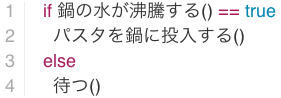
\includegraphics[width=.4\linewidth,bb=0 0 281 98]{images/background_cooking.js.png}
  \end{center}
  \caption{料理レシピをコンピュータプログラム風に記述する}
  \label{fig:background_cooking}
\end{figure}

また、小売店の店員マニュアルであれば、図\ref{fig:background_retail}のようになる

\begin{figure}[htbp]
  \begin{center}
  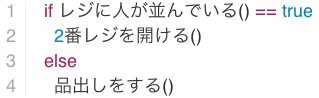
\includegraphics[width=.4\linewidth,bb=0 0 319 98]{images/background_retail.js.png}
  \end{center}
  \caption{料理レシピをコンピュータプログラム風に記述する}
  \label{fig:background_retail}
\end{figure}

このように、人間にとっての処理もコンピュータにとっての処理も、類似の記法で記述することが可能である。
プログラムは、コンピュータへの指示のようなものにだけに限定されない、より汎用的な処理の記述が可能なフォーマットである。

人間への指示をメインとしたプログラミングパラダイムによって、より人々の生活をコンピュータによる支援を受けたものにできる。
そもそも、人間とコンピュータでは得意分野や実現可能な処理が異なる。
人間は柔軟な思考能力や身体を所有することから、パターン認識や感性判断の必要な処理、実世界への干渉が得意である。
また、意思決定は基本的に人間が担うべき処理である。
コンピュータは高速な演算能力を有することから、計算や記憶、正確なセンシングなどを担うべきである。
人間にとってのタスクをプログラムとして記述し、コンピュータでも出来ることやコンピュータのほうが得意なことに関しては
コンピュータに実行させ、人間は人間にしかできないことや人間のほうが得意なことに専念する。
こういった、人間の行動を定義しつつ、コンピュータによる支援を受けることができれば、人間の行動はより効率的になったり、
良いものになるのではないかと考えられる。

このようなプログラミングパラダイムを実現することができれば、非常に面白い。
だが、現状では部分的にしか実現できていない。
プログラムから人間を計算資源として活用する仕組みは、主に知的労働への応用となっている。
人間の実世界での活動などを想定したものではない。
また、クラウドソーシング等の場合、インターネットを介した不特定の人間を対象としたものである。
自分の家で、自分の日常行動をプログラムにしたいとき等は、自分自身を対象として指定できなくてはならない。
また、家族等の身内にしか実行してほしくない処理の内容も存在することから、クラウドソーシング等の枠組みを利用することはできない。

そこで、本研究では、コンピュータと人間への指示を融合させたプログラミングが可能な環境を実現する。

\section{まとめ}\label{ux307eux3068ux3081}

本章では、プログラムの現状について示し、人間とコンピュータが対等な処理実行のリソースであるということを示した。
また、プログラムが実行対象を選ばない汎用的な処理記述フォーマットであることを示し、あらゆる処理を記述するためのプログラミング環境の実現に向けた
状況を考察した。
